% Created 2019-04-29 一 15:18
% Intended LaTeX compiler: pdflatex
\documentclass[11pt]{article}
\usepackage[utf8]{inputenc}
\usepackage[T1]{fontenc}
\usepackage{graphicx}
\usepackage{grffile}
\usepackage{longtable}
\usepackage{wrapfig}
\usepackage{rotating}
\usepackage[normalem]{ulem}
\usepackage{amsmath}
\usepackage{textcomp}
\usepackage{amssymb}
\usepackage{capt-of}
\usepackage{hyperref}
\usepackage{minted}
% TIPS
% \substack{a\\b} for multiple lines text





% pdfplots will load xolor automatically without option
\usepackage[dvipsnames]{xcolor}

\usepackage{forest}
% two-line text in node by [two \\ lines]
% \begin{forest} qtree, [..] \end{forest}
\forestset{
  qtree/.style={
    baseline,
    for tree={
      parent anchor=south,
      child anchor=north,
      align=center,
      inner sep=1pt,
    }}}
%\usepackage{flexisym}
% load order of mathtools and mathabx, otherwise conflict overbrace

\usepackage{mathtools}
%\usepackage{fourier}
\usepackage{pgfplots}
\usepackage{amsthm}
\usepackage{amsmath}
%\usepackage{unicode-math}
%
\usepackage{commath}
%\usepackage{,  , }
\usepackage{amsfonts}
\usepackage{amssymb}
% importing symbols https://tex.stackexchange.com/questions/14386/importing-a-single-symbol-from-a-different-font
%mathabx change every symbol
% use instead stmaryrd
%\usepackage{mathabx}
\usepackage{stmaryrd}
\usepackage{empheq}
\usepackage{tikz}
\usepackage{tikz-cd}
%\usepackage[notextcomp]{stix}
\usetikzlibrary{arrows.meta}
\usepackage[most]{tcolorbox}
%\utilde
%\usepackage{../../latexpackage/undertilde/undertilde}
% left and right superscript and subscript
\usepackage{actuarialsymbol}
\usepackage{threeparttable}
\usepackage{scalerel,stackengine}
\usepackage{stackrel}
% \stackrel[a]{b}{c}
\usepackage{dsfont}
% text font
\usepackage{newpxtext}
%\usepackage{newpxmath}

%\newcounter{dummy} \numberwithin{dummy}{section}
\newtheorem{dummy}{dummy}[section]
\theoremstyle{definition}
\newtheorem{definition}[dummy]{Definition}
\newtheorem{corollary}[dummy]{Corollary}
\newtheorem{lemma}[dummy]{Lemma}
\newtheorem{proposition}[dummy]{Proposition}
\newtheorem{theorem}[dummy]{Theorem}
\theoremstyle{definition}
\newtheorem{example}[dummy]{Example}
\theoremstyle{remark}
\newtheorem*{remark}{Remark}


\newcommand\what[1]{\ThisStyle{%
    \setbox0=\hbox{$\SavedStyle#1$}%
    \stackengine{-1.0\ht0+.5pt}{$\SavedStyle#1$}{%
      \stretchto{\scaleto{\SavedStyle\mkern.15mu\char'136}{2.6\wd0}}{1.4\ht0}%
    }{O}{c}{F}{T}{S}%
  }
}

\newcommand\wtilde[1]{\ThisStyle{%
    \setbox0=\hbox{$\SavedStyle#1$}%
    \stackengine{-.1\LMpt}{$\SavedStyle#1$}{%
      \stretchto{\scaleto{\SavedStyle\mkern.2mu\AC}{.5150\wd0}}{.6\ht0}%
    }{O}{c}{F}{T}{S}%
  }
}

\newcommand\wbar[1]{\ThisStyle{%
    \setbox0=\hbox{$\SavedStyle#1$}%
    \stackengine{.5pt+\LMpt}{$\SavedStyle#1$}{%
      \rule{\wd0}{\dimexpr.3\LMpt+.3pt}%
    }{O}{c}{F}{T}{S}%
  }
}

\newcommand{\bl}[1] {\boldsymbol{#1}}
\newcommand{\Wt}[1] {\stackrel{\sim}{\smash{#1}\rule{0pt}{1.1ex}}}
\newcommand{\wt}[1] {\widetilde{#1}}
\newcommand{\tf}[1] {\textbf{#1}}


%For boxed texts in align, use Aboxed{}
%otherwise use boxed{}

\DeclareMathSymbol{\widehatsym}{\mathord}{largesymbols}{"62}
\newcommand\lowerwidehatsym{%
  \text{\smash{\raisebox{-1.3ex}{%
    $\widehatsym$}}}}
\newcommand\fixwidehat[1]{%
  \mathchoice
    {\accentset{\displaystyle\lowerwidehatsym}{#1}}
    {\accentset{\textstyle\lowerwidehatsym}{#1}}
    {\accentset{\scriptstyle\lowerwidehatsym}{#1}}
    {\accentset{\scriptscriptstyle\lowerwidehatsym}{#1}}
}

\usepackage{graphicx}
    
% text on arrow for xRightarrow
\makeatletter
%\newcommand{\xRightarrow}[2][]{\ext@arrow 0359\Rightarrowfill@{#1}{#2}}
\makeatother


\newcommand{\dom}[1]{%
\mathrm{dom}{(#1)}
}

% Roman numerals
\makeatletter
\newcommand*{\rom}[1]{\expandafter\@slowromancap\romannumeral #1@}
\makeatother

\def \fR {\mathfrak{R}}
\def \bx {\boldsymbol{x}}
\def \bz {\boldsymbol{z}}
\def \ba {\boldsymbol{a}}
\def \bh {\boldsymbol{h}}
\def \bo {\boldsymbol{o}}
\def \bU {\boldsymbol{U}}
\def \bc {\boldsymbol{c}}
\def \bV {\boldsymbol{V}}
\def \bI {\boldsymbol{I}}
\def \bK {\boldsymbol{K}}
\def \bt {\boldsymbol{t}}
\def \bb {\boldsymbol{b}}
\def \bA {\boldsymbol{A}}
\def \bX {\boldsymbol{X}}
\def \bu {\boldsymbol{u}}
\def \bS {\boldsymbol{S}}
\def \bZ {\boldsymbol{Z}}
\def \bz {\boldsymbol{z}}
\def \by {\boldsymbol{y}}
\def \bw {\boldsymbol{w}}
\def \bT {\boldsymbol{T}}
\def \bF {\boldsymbol{F}}
\def \bS {\boldsymbol{S}}
\def \bm {\boldsymbol{m}}
\def \bW {\boldsymbol{W}}
\def \bR {\boldsymbol{R}}
\def \bQ {\boldsymbol{Q}}
\def \bS {\boldsymbol{S}}
\def \bP {\boldsymbol{P}}
\def \bT {\boldsymbol{T}}
\def \bY {\boldsymbol{Y}}
\def \bH {\boldsymbol{H}}
\def \bB {\boldsymbol{B}}
\def \blambda {\boldsymbol{\lambda}}
\def \bPhi {\boldsymbol{\Phi}}
\def \btheta {\boldsymbol{\theta}}
\def \bTheta {\boldsymbol{\Theta}}
\def \bmu {\boldsymbol{\mu}}
\def \bphi {\boldsymbol{\phi}}
\def \bSigma {\boldsymbol{\Sigma}}
\def \lb {\left\{}
\def \rb {\right\}}
\def \la {\langle}
\def \ra {\rangle}
\def \caln {\mathcal{N}}
\def \dissum {\displaystyle\Sigma}
\def \dispro {\displaystyle\prod}
\def \E {\mathbb{E}}
\def \Q {\mathbb{Q}}
\def \N {\mathbb{N}}
\def \V {\mathbb{V}}
\def \R {\mathbb{R}}
\def \P {\mathbb{P}}
\def \A {\mathbb{A}}
\def \Z {\mathbb{Z}}
\def \I {\mathbb{I}}
\def \C {\mathbb{C}}
\def \cala {\mathcal{A}}
\def \calb {\mathcal{B}}
\def \calq {\mathcal{Q}}
\def \calp {\mathcal{P}}
\def \cals {\mathcal{S}}
\def \calg {\mathcal{G}}
\def \caln {\mathcal{N}}
\def \calr {\mathcal{R}}
\def \calm {\mathcal{M}}
\def \calc {\mathcal{C}}
\def \calf {\mathcal{F}}
\def \calk {\mathcal{K}}
\def \call {\mathcal{L}}
\def \calu {\mathcal{U}}
\def \bcup {\bigcup}


\def \uin {\underline{\in}}
\def \oin {\overline{\in}}
\def \uR {\underline{R}}
\def \oR {\overline{R}}
\def \uP {\underline{P}}
\def \oP {\overline{P}}

\def \Ra {\Rightarrow}

\def \e {\enspace}

\def \sgn {\operatorname{sgn}}
\def \gen {\operatorname{gen}}
\def \ker {\operatorname{ker}}
\def \im {\operatorname{im}}

\def \tril {\triangleleft}

% \varprod
\DeclareSymbolFont{largesymbolsA}{U}{txexa}{m}{n}
\DeclareMathSymbol{\varprod}{\mathop}{largesymbolsA}{16}

% \bigtimes
\DeclareFontFamily{U}{mathx}{\hyphenchar\font45}
\DeclareFontShape{U}{mathx}{m}{n}{
      <5> <6> <7> <8> <9> <10>
      <10.95> <12> <14.4> <17.28> <20.74> <24.88>
      mathx10
      }{}
\DeclareSymbolFont{mathx}{U}{mathx}{m}{n}
\DeclareMathSymbol{\bigtimes}{1}{mathx}{"91}
% \odiv
\DeclareFontFamily{U}{matha}{\hyphenchar\font45}
\DeclareFontShape{U}{matha}{m}{n}{
      <5> <6> <7> <8> <9> <10> gen * matha
      <10.95> matha10 <12> <14.4> <17.28> <20.74> <24.88> matha12
      }{}
\DeclareSymbolFont{matha}{U}{matha}{m}{n}
\DeclareMathSymbol{\odiv}         {2}{matha}{"63}


\newcommand\subsetsim{\mathrel{%
  \ooalign{\raise0.2ex\hbox{\scalebox{0.9}{$\subset$}}\cr\hidewidth\raise-0.85ex\hbox{\scalebox{0.9}{$\sim$}}\hidewidth\cr}}}
\newcommand\simsubset{\mathrel{%
  \ooalign{\raise-0.2ex\hbox{\scalebox{0.9}{$\subset$}}\cr\hidewidth\raise0.75ex\hbox{\scalebox{0.9}{$\sim$}}\hidewidth\cr}}}

\newcommand\simsubsetsim{\mathrel{%
  \ooalign{\raise0ex\hbox{\scalebox{0.8}{$\subset$}}\cr\hidewidth\raise1ex\hbox{\scalebox{0.75}{$\sim$}}\hidewidth\cr\raise-0.95ex\hbox{\scalebox{0.8}{$\sim$}}\cr\hidewidth}}}
\newcommand{\stcomp}[1]{{#1}^{\mathsf{c}}}


\graphicspath{{../../images/NumericalAnalysis/}}
\author{gouziwu}
\date{\today}
\title{Numerical Analysis}
\hypersetup{
  pdfauthor={gouziwu},
  pdftitle={Numerical Analysis},
  pdfkeywords={},
  pdfsubject={},
  pdfcreator={Emacs 26.1 (Org mode 9.1.14)}, 
  pdflang={English}}
\begin{document}

\maketitle
\tableofcontents


\section{Chap1 Mathematical Preliminaries}
\label{sec:orgdf9a8e9}
\subsection{1.2 Roundoff Errors and Computer Arithmetic}
\label{sec:org8e7a348}
\textbf{Truncation Error} : the error involved in using a truncated, or finite, summation to
approximate the sum of an infinite series 

\textbf{Roundoff Error}: the error produced when performing real number calculations.
It occurs because the arithmetic performed in a machine involves numbers
with only a finite number of digits. 


Suppose \(y=\textcolor{blue}{0.d_1d_2\dots
  d_k}d_{k+1}d_{k+2}\dots\textcolor{blue}{\times 10^n{}}\), then

\(fl(y)=\begin{cases} 0.d_1d_2\dots d_k\times 10^n&\quad\text{chopping}\\
  chop(y+5\times 10^{n-(k+1)})=0.\delta_1\delta_2\dots \delta_k\times
  10^n&\quad\text{Rounding}\\\end{cases}\)


\begin{definition}
  If $p*$ is an approximation to $p$, the \textcolor{red}{absolute error} is $|p-p*|$,
  and the \textcolor{red}{relative error} is $\frac{|p-p*|}{|p|}$, provided that $p\neq 0$
\end{definition}

\begin{definition}
  The number $p*$ is said to approximate $p$ to $t$
  \textcolor{red}{significant digits} if $t$ is the largest nonnegative
  integer for which $\frac{|p-p*|}{|p|}<5\times 10^{-t}$
\end{definition}

\begin{description}
\item[{chopping}] \(|\frac{y-fl(y)}{y}|=|\frac{0.d_1d_2\dots d_kd_{k+1}\dots
    \times 10^n-0.d_1d_2\dots d_k\times 10^n}{0.d_1d_2\dots
    d_kd_{k+1}\times
    10^n}|=|\frac{0.d_{k+1}\dots}{0.d_1d_2\dots}|\times 10^{-k}\le
  \frac{1}{0.1}\times 10^{-k}=10^{-k+1}\)
\item[{rounding}] \(|\frac{y-fl(y)}{y}|\le \frac{0.5}{0.1}\times 10^{-k}=0.5\times
  10^{-k+1}\)
\end{description}

\textbf{Finite digit arithmetic}

\begin{itemize}
\item \(x\oplus y=fl(fl(x)+fl(y))\)
\item \(x\otimes y=fl(fl(x)\times fl(y))\)
\item \(x\ominus y=fl(fl(x)-fl(y))\)
\item \(x\odiv y=fl(fl(x)\div fl(y))\)
\end{itemize}

\subsection{1.3 ALgorithms and Convergence}
\label{sec:org5e56c3e}
An algorithm that satisfies that small changes in the initial data produce
correspondingly small changes in the final results is called \textbf{stable};
otherwise it is \textbf{unstable}. An algorithm is called \textbf{conditionally stable} if it
is stable only for certain choices of initial data. 

Suppose that E₀ > 0 denotes an initial error and En represents the magnitude
of an error after n subsequent operations. If \(E_n\approx CnE_0\), where C is a
constant independent of n, then the growth of error is said to be \textbf{linear}. If
\(E_n\approx C^nE_0\), for some C > 1, then the growth of error is called \textbf{exponential} 

Suppose \(\{\beta_n\}_{n=1}^\infty, \lim\limits_{n \to \infty}\beta_n=0,
\{\alpha_n\}_{n=1}^\infty, \lim\limits_{n\to\infty}\alpha_n=\alpha\).
If a positive constant K exists with \(|\alpha_n-\alpha|\le K|\beta_n|\) for
large n, then \(\{\alpha_n\}_{n=1}^\infty\) converges to α with \textbf{rate, or}
\textbf{order, of convergence} \(O(\beta_n)\)

Suppose \(\lim\limits_{h\to 0}G(h)=0, \lim\limits_{h\to 0}F(h)=L\) and
\(|F(h)-L|\le K|G(h)|\) for sufficiently small h, then we write
\(F(h)=L+O(G(h))\)
\section{Chap2 Solutions of equations in one variable}
\label{sec:org50b42ef}
\subsection{2.1 Bisection method}
\label{sec:orgca05e0d}
\begin{theorem}{Intermediate Value Theorem}
  If $f\in C[a,b]$, $K\in(f(a), f(b))$, then there exists a number $p\in(a,b)$
  for which $f(p)=K$
\end{theorem}

\begin{theorem}
  Suppose that $f\in C[a,b]$ and $f(a)\cdot f(b)<0$. The bisection method
  generates a sequence $\{p_n\},n=0,1,\dots$ approximating a zero $p$ of $f$ with
  \begin{equation*}
    |p_n-p|\le\frac{b-a}{2^n}, \quad\text{when } n\ge 1
  \end{equation*}
\end{theorem}
\subsection{2.2 Fixed-Point Iteration}
\label{sec:org5e0d4bc}
\(f(x)=0\xleftrightarrow{\text{equivalent}} x=f(x)+x=g(x)\)

\begin{theorem}{Fixed-Point Theorem}
  Let $g\in C[a,b]$ be s.t. $g(x)\in[a,b]$ for all $x\in[a,b]$. Suppose that
  $g'$ exists on $(a,b)$ and that a constant $0<k<1$ exists with $|g'(x)|\le k$
  for all $x\in(a,b)$ (hence $g'$ can't converge to 1). Then for any number
  $p_0$ in $[a,b]$, the sequence defined by $p_n=g(p_{n-1}), n\ge 1$ converges
  to the unique point $p$ in $[a,b]$
\end{theorem}

\begin{corollary}
  $|p_n-p|\le\frac{1}{1-k}|p_{n+1}-p_n|$ and
  $|p_n-p|\le\frac{k^n}{1-k}|p_1-p_0|$
\end{corollary}
\subsection{2.3 Newton's method}
\label{sec:org4280124}
Linearize a nonlinear function using \textbf{Taylor's expansion}

Let \(p_0\in [a,b]\) be an approximation to \(p\) s.t. \(f'(p_0)\neq 0\), hence 
\(f(x)=f(p_0)+f'(p_0)(x-p_0)+\frac{f''(\xi_x)}{2!}(x-p_0)^2\), then
\(0=f(p)\approx f(p_0)+f'(p_0)(p-p0)\rightarrow p\approx
p_0-\frac{f(p_0)}{f'(p_0)}\)
\(p_n=p_{n-1}-\frac{f(p_{n-1})}{f'(p_{n-1})},\quad\text{for} n\ge 1\)

\begin{theorem}
  Let $f\in C^2[a,b]$. If $p\in[a,b]$ is s.t. $f(p)=0,f'(p)\neq0$, then there
  exists a $\delta>0$ s.t. Newton's method generates a sequence $\{p_n\},
  n\in\mathbb{N}\setminus\{0\}$ converging to $p$ for any initial approximation
  $p\in[p-\delta,p+\delta]$.
\end{theorem}
\subsection{2.4 Error analysis for iterative methods}
\label{sec:orge44982f}
\begin{definition}
  Suppose $\{p_n\}(n=0,1,\dots)$ is a sequence that converges to $p$ with
  $p_n\neq p$ for all $n$. If positive constants $\alpha$ and $\lambda$ exist
  with
  \begin{equation*}
    \lim\limits_{n\to\infty}\frac{|p_{n+1}-p|}{|p_n-p|^\alpha}=\lambda
  \end{equation*}
  then $\{p_n\}(n=0,1,\dots)$ \textcolor{red}{converges to p of order
    $\alpha$, with asymptotic error constant $\lambda$}
\end{definition}

\begin{theorem}
  Let $p$ be a fixed point of $g(x)$. If there exists some constant $\alpha\ge
  2$ s.t. $g\in C^\alpha[p-\delta,p+\delta]$,
  \textcolor{red}{$g'(p)=\dots=g^{\alpha-1}(p)=0$} and \textcolor{red}{$g^\alpha(p)\neq 0$}.
  Then the iterations with $p_n=g(p_{n-1})$, $n\ge1$ is of \textcolor{red}{order $\alpha$}
\end{theorem}

\begin{equation*}
  p_{n+1}=g(p_n)=g(p)+g'(p)(p_n-p)+\dots+\frac{g^\alpha(\xi_n)}{\alpha!}(p_n-p)^\alpha
\end{equation*}

\begin{theorem}
  Let $g\in C[a,b]$ be s.t. $g(x)\in[a,b]$ for all $x\in[a,b]$. Suppose in
  addition that $g'$ is continuous on $(a,b)$ and a positive constant $k<1$
  exists with
  \begin{equation*}
    |g'(x)|\le k, \quad \text{for all } x\in(a,b)
  \end{equation*}
  If $g'(p)\neq0$, then for any number $p_0\neq p$ in $[a,b]$, the sequence
  \begin{equation*}
    p_n=g(p_{n-1}),\quad\text{for }n\ge 1
  \end{equation*}
  converges only linearly to the unique fixed point in $[a,b]$
\end{theorem}

\begin{proof}
  \begin{align*}
    \lim\limits_{n\to\infty}\frac{|p_{n+1}-p|}{|p_n-p|}&=
                                                         \lim\limits_{n\to\infty}\frac{|g(p_n)-p|}{|p_n-p|}\\
                                                       &=\lim\limits_{n\to\infty}\frac{|g'(\xi)(p_n-p)|}{|p_n-p|}\\
                                                       &=|g'(p)|
  \end{align*}
\end{proof}

\begin{theorem}
  Let $p$ be a solution of the equation $x=g(x)$. Suppose that $g'(p)=0$ and
  g'' is continuous with $|g''(x)|<M$ on an open interval $I$ containing $p$.
  Then there exists a $\delta>0$ s.t. for $p_0\in[p-\delta,p+\delta]$, the
  sequence defined by $p_n=g(p_{n-1})$, when $n\ge 1$ converges at least
  quadratically to $p$. Moreover, for sufficiently large values of $n$,
  \begin{equation*}
    |p_{n+1}-p|<\frac{M}{2}|p_n-p|^2
  \end{equation*}
\end{theorem}

\begin{proof}
  Choose $k\in(0,1),\delta>0$ s.t. $[p-\delta,p+\delta]\subseteq I$ and
  $|g'(x)|<k$ and $g''$ is continuous.
  \begin{equation*}
    g(x)=g(p)+g'(p)(x-p)+\frac{g''(\xi)}{2}(x-p)^2
  \end{equation*}
  Hence $g(x)=p+\frac{g''(\xi)}{2}(x-p)^2$.
  $p_{n+1}=g(p_n)=p+\frac{g''(\xi_n)}{2}(p_n-p)^2$. Thus
  $p_{n+1}-p=\frac{g''(\xi_n)}{2}(p_n-p)^2$. We get
  \begin{equation*}
    \lim\limits_{n\to\infty}\frac{|p_{n+1}-p|}{|p_n-p|^2}=\frac{g''(p)}{2}
  \end{equation*}
\end{proof}

\begin{definition}
  A solution $p$ of $f(x) = 0$ is a \textcolor{red}{zero of multiplicity} $m$
  of $f$ if for $x\neq p$, $f(x)=(x-p)^mq(x)$ where $\lim\limits_{x\to
    p}q(x)\neq 0$
\end{definition}

\begin{theorem}
  The function $f\in C^m[a,b]$ has a zero of multiplicity $m$ at $p$ in $(a,b)$
  if and only if
  \begin{equation*}
    0=f(p)=f'(p)=\dots=f^{(m-1)}(p),\quad\text{but } f^{(m)}(p)\neq 0
  \end{equation*}
\end{theorem}

To handle the problem of multiple roots of a function \(f\) is to define
\(\mu(x)=\frac{f(x)}{f'(x)}\).

If p is a zero of f of multiplicity m with \(f(x)=(x-p)^mq(x
)\), then
\begin{align*}
  \mu(x)&=\frac{(x-p)^mq(x)}{m(x-p)^{m-1}q(x)+(x-p)^mq'(x)}\\
        &=(x-p)\frac{q(x)}{mq(x)+(x-p)q'(x)}
\end{align*}
And \(q(x)\neq 0\).

Now Newton's method:
\begin{align*}
  g(x)&=x-\frac{\mu(x)}{\mu'(x)}\\
      &=x-\frac{f(x)/f'(x)}{(f'(x)^2-f(x)f''(x))/f'(x)^2}\\
      &=x-\frac{f(x)f'(x)}{f'(x)^2-f(x)f''(x)}
\end{align*}
\section{Chap3 Interpolation and polynomial approximation}
\label{sec:orge481c06}
\subsection{3.1 Interpolation and the Lagrange polynomial}
\label{sec:org4249e8b}
\(P_n(x)=\displaystyle\sum_{i=0}^nL_{n,i}(x)y_i\). Find \(L_{n,i}(x)\) for
\(i=0,\dots,n\) s.t. \(L_{n,j}(x_j)=\delta_{ij}\). \(\delta_{ij}\) Kronecker delta.
Each \(L_{n,i}\) has n roots \(x_0,\dots,\hat{x_i},\dots,x_n\).
\(L_{n,j}(x)=C_i(x-x_0)\dots\hat{(x-x_i)}\dots(x-x_n)=C_i \displaystyle
\prod_{\substack{j\neq i\\j=0}}^n(x-x_j)\).
\(L_{n,j}(x_i)=1\to C_i=\displaystyle\prod_{j\neq i}\frac{1}{x_i-x_j}\).
Hence \(L_{n,i}(x)=\displaystyle\prod_{\substack{j\neq i\\j=0}}^n
\frac{x-x_j}{x_i-x_j}\)

\begin{theorem}
  If $x_0,x_1,\dots,x_n$ are n+1 distinct numbers and $f$ is a function whose values
  are given at these numbers, then the n-th Lagrange interpolating polynomial 
  is unique
\end{theorem}


\textbf{Analyze the remainder}. Suppose \(a\le x_0<x_1<\dots<x_n\le b\) and \(f\in
C^{n+1}[a,b]\). Consider \(R_n(x)=f(x)-P_n(x)\).
\(R_n(x)\) has at least n+1 roots =>
\(R_n(x)=K(x)\displaystyle\prod_{i=0}^n(x-x_i)\).
For any \(x\neq x_i\). Define
\(g(t)=R_n(t)-K(x)\displaystyle\prod_{i=0}^n(t-x_i)\). \(g(x)\) has n+2 distinct
roots \(x_0\dots x_n x\). Hence \(g^{(n+1)}(\xi_x)=0,\xi_x\in(a,b)\).
\(f^{(n+1)}(\xi_x)-Pn^{(n+1)}(\xi_x)-K(x)(n+1)!=R_n^{(n+1)}(\xi_x)-K(x)(n+1)!\).
Thus
\(R_n(x)=\frac{f^{(n+1)}(\xi_x)}{(n+1)!}\displaystyle\prod_{i=0}^n(x-x_i)\).

\begin{definition}
  Let $f$ be a function defined at $x_0,\dots,x_n$ and suppose $m_1,\dots,m_k$ are
  k distinct integers with $0\le m_i\le n$ for each i. The Lagrange polynomial that
  agrees with $f(x)$ at the k points $x_{m_1},\dots,x_{m_k}$ denoted by 
  $P_{m_1,\dot,m_k}(x)$
\end{definition}

\begin{theorem}
  Let $f$ be defined at $x_0,\dots,x_k$ and let $x_i$ and $x_j$ be two distinct numbers in
  this set. Then
  \begin{equation*}
    P(x)=\frac{(x-x_j)P_{0,1,\dots,j-1,j+1,\dots,k(x)}-(x-x_i)P_{0,\dots,i-1,i+1,\dots,k(x)}}
    {x_i-x_j}
  \end{equation*}
  describes the k-th Lagrange polynomial that interpolates $f$ at the k+1 points
  $x_0,\dots,x_k$
\end{theorem}

\textbf{Neville's Method}
n   \begin{tabular}{c c c c c c}
      \(x_0\) \& \(P_0\) \&           \&             \&            \\
      \(x_1\) \& \(P_1\) \& \(P_{0,1}\) \&             \&            \\
      \(x_2\) \& \(P_2\) \& \(P_{1,2}\) \& \(P_{0,1,2}\) \&            \\
      \(x_3\) \& \(P_3\) \& \(P_{2,3}\) \& \(P_{1,2,3}\) \& \$P\(_{\text{0,1,2,3}}\)\$\\
    \end{tabular}n
    \subsection{3.2 Divied differences}
    \label{sec:org1bd045f}
    \(f[x_i,x_j]=\frac{f(x_i)-f(x_j)}{x_i-x_j}(i\neq j, x_i\neq x_j)\).
    \(f[x_i,x_j,x_k]=\frac{f[x_i,x_j]-f[x_j,x_k]}{x_i-x_k}\).
    \subsection{Additional Newton Interpolation}
    \label{sec:orgcac1df0}
    \subsubsection{Simple idea}
    \label{sec:org97b005e}
    Given \(x_0,\dots,x_n\)
    \begin{enumerate}
    \item Fitting $x_0$ first: $f(x)\approx f_0, f_0=f(x_0)$
    \item Add one more point $x_1$, $f_1=f(x_1)$
      \begin{equation*}
        f(x) \approx f_0+\alpha_1(x-x_0),\alpha_1=\frac{f_1-f_0}{x_1-x_0}
      \end{equation*}
    \item More points $f(x)\approx f_0+\alpha_1(x-x_0)+\alpha_2(x-x_0)(x-x_1)$
    \end{enumerate}

    \textbf{The pattern and coefficients}.
    \(f(x)=\displaystyle\sum_{i=0}^n\alpha_i
    \displaystyle\prod_{j=0}^{j<i}(x-x_j)
    =\displaystyle\sum_{i=0}^n\alpha_iN^{(i)}(x)\)

    \begin{equation*}
      \begin{pmatrix}
        f_0\\
        f_1\\
        \vdots\\
        f_n
      \end{pmatrix}=
      \begin{pmatrix}
        N^{(0)}(x_0) & N^{(1)}(x_0) & \dots & N^{(n)}(x_0)\\
        N^{(0)}(x_1) & N^{(1)}(x_1) & \dots & N^{(n)}(x_1)\\
        \vdots & \vdots & \ddots&\vdots\\
        N^{(0)}(x_n) & N^{(1)}(x_n) & \dots & N^{(n)}(x_n)\\
      \end{pmatrix}
      \begin{pmatrix}
        \alpha_0\\
        \alpha_1\\
        \vdots\\
        \alpha_n
      \end{pmatrix}
    \end{equation*}

    \(N^{(i)}(x_k)=\begin{cases}
      0&k<i\\
      \prod_{j=0}^{j<i}(x_k-x_j)&k\ge i\\
    \end{cases}\) with \(N^{(0)}(x) = 1\).
    Newton interpolation matrix is lower triangular.
    Lagrange matrix is identity.
    \subsubsection{Basis transformation}
    \label{sec:org32b4e0b}
    \begin{equation*}
      \begin{pmatrix}
        1\\
        (x-x_0)\\
        (x-x_0)(x-x_1)\\
        \vdots
      \end{pmatrix}=(?)
      \begin{pmatrix}
        1\\
        x\\
        x^2\\
        \vdots
      \end{pmatrix}
    \end{equation*}
    Hence \((\Phi_B)^T=(T_A^B)^T(\Phi_A)^T\).
    \(\Phi_B=\Phi_AT_A^B\)

    \begin{align*}
      (\Phi_A)(\alpha_A)=(f)&=(\Phi_B)(\alpha_B)\\
                            &=(\Phi_A)(T_A^B)(\alpha_B)\\
                            &\Rightarrow\\
      (\alpha_A)&=(T_A^B)(\alpha_B)\\
      (\alpha_B)&=(T_A^B)^{-1}(\alpha_A)\\
                            &=(T_B^A)(\alpha_A)
    \end{align*}
    \subsection{3.3 Hermite interpolation}
    \label{sec:org5ca591b}
    Find the \textbf{osculating polynomial} \(P(x)\) s.t. \(P(x_i)=f(x_i),
    P'(x_i)=f'(x_i),\dots,P^{(m_i)}(x_i)=f^{(m_i)}(x_i)\) for all \(i=0,1,\dots,n\).

    Just the Taylor polynomial \(P(x)=f(x_0)+f'(x_0)(x-x_0)+\dots+
    \frac{f^{(m_0)}(x_0)}{m_0!}(x-x_0)^{m_0}\) with remainder 
    \(R(x)=f(x)-\varphi(x)=\frac{f^{(m_0+1)}(\xi)}{(m_0+1)!}(x-x_0)^{(m_0+1)}\)

    \(m_i = 1\) gives \textbf{Hermite polynomial}

    \begin{example}
      Suppose $x_0\neq x_1\neq x_2$. Given $f(x_0),f(x_1), f(x_2),
      f'(x_1)$ find the polynomial $P(x)$ s.t. $P(x_i)=f(x_i),P'(x_1)=f'(x_1)$ and
      analyze the errors.
    \end{example}

    \begin{proof}
      $P_3(x)=\displaystyle\sum_{i=0}^2f(x_i)h_i(x)+f'(x_1)\hat{h}_1(x)$ where
      $h_i(x_j)=\delta_{ij},h_i'(x_i)=0,\hat{h}_i(x_i)=0,\hat{h}_i'(x_1)=1$.
      \begin{itemize}
      \item $h_0(x)$. Has roots $x_1,x_2$ and $x_1$ is a multiple root.
        $h_0(x)=C_0(x-x_1)^2(x-x_2)$ and $h_0(x_0)=1\Longrightarrow C_0$
      \item $\hat{h}_1(x)$ has root $x_0,x_1,x_2\Longrightarrow 
        \hat{h}_1(x)=C_1(x-x_0)(x-x_1)(x-x_2)$
      \end{itemize}
    \end{proof}

    In general, given \(x_0,\dots,x_n;y_0,\dots,y_n\) and \(y_0',\dots,y_n'\). The
    Hermite polynomial \(H_{2n+1}(x)\) satisfies \(H_{2n+1}(x_i)=y_i\) and
    \(H'_{2n+1}(x_i)=y_i'\) 

    \emph{Solution}.
    \(H_{2n+1}(x)=\displaystyle\sum_{i=0}^ny_ih_i(x)+\displaystyle\sum_{i=0}^ny_i'
    \hat{h}_i(x)\)
    \subsection{3.4 Cubic spline interpolation}
    \label{sec:org1999dd5}
    \textbf{Piecewise linear interpolation}. Approximate \(f(x)\) by linear polynomials on
    each subinterval \([x_i,x_{i+1}]\).

    \(f\approx P_1(x)=\frac{x-x_{i+1}}{x_i-x_{i+1}}y_i+\frac{x-x_i}
    {x_{i+1}-x_i}y_{i+1} \quad\text{for} \;x\in[x_i,x_{i+1}]\) 

    Let \(h=\max\abs{x_{i+1}-x_i}\). Then \(P_1^h(x)\xrightarrow{uniform} f(x)\) as
    \(h\to 0\) 
    However, this is no longer smooth.

    \textbf{Hermite piecewise polynomials}. Given
    \(x_0,\dots,x_n;y_0,\dots,y_n,y_0',\dots,y_n'\), construct the Hermite
    polynomial of degree 3 with \(y\) and \(y'\) on the two endpoints of
    \([x_i,x_{i+1}]\)

    \textbf{Cubic Spline}.
    \begin{definition}
      Given a function $f$ define on $[a,b]$ and a set of nodes $a=x_0<x_1<\dots<x_n=b$,
      \textcolor{red}{cubic spline interpolant} $S$ for $f$ is a function that satisfies
      the following conditions
      \begin{itemize}
      \item $S(x)$ is a cubic polynomial, denoted by $S_i(x)$ on the subinterval
        $[x_i,x_{i+1}]$ for each $i=0,\dots,n-1$
      \item $S(x_i)=f(x_i)$ for each $i=0,\dots, n$
      \item $S_{i+1}(x_{i+1})=S_i(x_{i+1})$
      \item $S'_{i+1}(x_{i+1})=S'_i(x_{i+1})$
      \item $S''_{i+1}(x_{i+1})=S''_i(x_{i+1})$
      \end{itemize}
    \end{definition}

    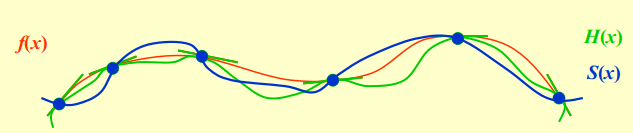
\includegraphics[width=100mm]{CubicSpline}

    \textbf{Method of Bending moment}. Let \(h_j=x_j-x_{j-1}\) and \(S(x)=S_j(x)\) for
    \(x\in[x_{j-1}, x_j]\). Then \(S_j''\) is a polynomial of degree
    \textcolor{red}{1}, which can be determined by the values of f on
    \textcolor{red}{2} nodes .

    Assume \(S_j''(x_{j-1})=M_{j-1},S_j''(x_j)=M_j\). Then for all
    \(x\in[x_{j-1},x_j]\),
    \(S_j''(x)=M_{j-1}\frac{x_j-x}{h_j}+M_j\frac{x-x_{j-1}}{h_j}\). Hence we get
    \begin{align*}
      &S_j'(x)=-M_{j-1}\frac{(x_j-x)^2}{2h_j}+M_j\frac{(x-x_{j-1})^2}{2h_j}+A_j\\
      &S_j(x)=M_{j-1}\frac{(x_j-x)^3}{6h_j}+M_j\frac{(x-x_{j-1})^3}{6h_j}+A_jx+B_j
    \end{align*}

    Solve this by \(S_j(x_{j-1})=y_{j-1},S_j(x_j)=y_j\), we get
    \begin{align*}
      A_j&=\frac{y_j-y_{j-1}}{h_j}-\frac{M_j-M_{j-1}}{6}h_j\\
      A_jx+B_j&=(y_{i-1}-\frac{M_{j-1}}{6}h_j^2)\frac{x_j-x}{h_j}+ 
                (y_j-\frac{M_j}{6}h_j^2)\frac{x-x_{j-1}}{h_j}
    \end{align*}

    Now solve for \(M_j\): Since \(S'\) is continuous at \(x_j\)
    \begin{align*}
      [x_{j-1},x_j]:S'_j(x)&=-M_{j-1}\frac{(x_j-x)^2}{2h_j}+M_j\frac{(x-x_{j-1})^2}{2h_j}
                             +f[x_{j-1},x_j]-\frac{M_j-M_{j-1}}{6}h_j\\
      [x_j,x_{j+1}]:S'_{j+1}(x)&=-M_j\frac{(x_{j+1}-x)^2}{2h_{j+1}}+M_{j+1}
                                 \frac{(x-x_j)^2}{2h_{j+1}}+f[x_j,x_{j+1}]-\frac{M_{j+1}-M_j}{6}h_{j+1}\\
    \end{align*}
    From \(S'_j(x_j)=S'_{j+1}(x_j)\), let \(\lambda_j=\frac{h_{j+1}}{h_j+h_{j+1}},
    \mu_j=1-\lambda_j,g_j=\frac{6}{h_j+h_{j+1}}(f[x_j,x_{j+1}]-f[x_{j-1},x_j])\)
    we get
    \begin{equation*}
      \mu_jM_{j-1}+2M_j+\lambda_jM_{j+1}=g_j\quad\text{for } \;1\le j\le n-1
    \end{equation*}
    \begin{equation*}
      \begin{pmatrix}
        \mu_1 & 2 & \lambda_1 &&\\
        & \ddots &\ddots &\ddots &\\
        &&\mu_{n-1}&2&\lambda_{n-1}
      \end{pmatrix}
      \begin{pmatrix}
        M_0\\
        \vdots\\
        \vdots\\
        M_n\\
      \end{pmatrix}=
      \begin{pmatrix}
        g_1\\
        \vdots\\
        g_{n-1}
      \end{pmatrix}
    \end{equation*}

    And \(S'(a)=y_0',S'(b)=y_n'\)

    \section{Chap6 Direct Methods for Solving Linear Systems}
    \label{sec:orgd8293a7}
    \subsection{6.1 Linear Systems of Equations}
    \label{sec:org3258375}
    \textbf{Gaussian elimination with backward substitution}
    \subsection{6.2 Pivoting Strategies}
    \label{sec:org07a6318}
    \textbf{Problem}: small pivot element may cause trouble

    \textbf{Paritial Pivoting}: Determine the smallest p≥k s.t.
    \(|a_{pk}^{(k)}|=\displaystyle\max_{k\le j\le n}|a_{ik}^{(k)}|\) and
    interchange the pth and the kth rows

    \textbf{Scaled Partial Pivoting}:
    \begin{enumerate}
    \item Define a scale factor \(s_i\) for each row as \(s_i=\displaystyle\max_{1\le
        j\le n}|a_{ij}|\)
    \item Determine the smallest \(p\ge k\) s.t.
      \(\frac{|a_{pk}^{(k)}}{s_p}=\displaystyle\max_{k\le i\le
        n}\frac{|a_{ik}^{(k)}|}{s_i}\)
      and interchange the pth and the kth rows
    \end{enumerate}


    \textbf{Complete Pivoting}: Search all the entries \(a_{ij}\) to find the entry with
    the largest magnitude
    \subsection{6.5 Matrix Factorization}
    \label{sec:org33daf6e}
    \(m_{ik}=a_{ik}/a_{kk}\)
    \begin{equation*}
      L_k=
      \begin{pmatrix}
        1 &            &            &               &  \\
        & \ddots     &            &\mbox{\Huge 0} &  \\
        &            & 1          &               &  \\
        &            & -m_{k+1,k} &               &  \\
        &            & \vdots     & \ddots        &  \\
        &            & -m_{n,k}   &               & 1\\
      \end{pmatrix}
    \end{equation*}  


    Hence 

    \begin{equation*}
      L_1^{-1}L_2^{-1}\dots L_{n-1}^{-1}=
      \begin{pmatrix}
        1&&&\mbox{\Huge 0}\\
        &1&&\\
        &&\ddots&\\
        \text{\Huge $m_{i,j}$}&&&1\\
      \end{pmatrix}
    \end{equation*}

    \begin{equation*}
      U=
      \begin{pmatrix}
        a_{11}&a_{12}&\dots&a_{1n}\\
        &a_{22}&\dots&a_{2n}\\
        &&\dots&\vdots\\
        &&&a_{nn}\\
      \end{pmatrix}
    \end{equation*}

    \(A=LU\)
    \subsection{6.6 Special Types of Matrices}
    \label{sec:org0a821ff}
    \textbf{Strictly Diagonally Dominant Matrix}.
    \(|a_{ii}|>\displaystyle\sum_{\substack{j=1,\\j\neq i}}^n|a_{ij}| \quad
    \text{for each } i=1,\dots,n\)

    \begin{theorem}
      A strictly diagonally dominant matrix A is \textcolor{red}{nonsingular}. Moreover,
      Gaussian elimination can be performed \textcolor{red}{without} row or column
      \textcolor{red}{interchanges}, and the computations will be \textcolor{red}{stable}
      w.r.t. the growth of roundoff errors
    \end{theorem}

    \textbf{Choleski's Method for Positive Definite Matrix}:
    \begin{definition}
      A matrix A is \textcolor{red}{positive definite} if ti's symmetric and if    
      $ \mathbf{x}^T \mathbf{A} \mathbf{x}>0$ for every n-dimensional vector $ \mathbf{x}\neq 0$
    \end{definition}

    \begin{lemma}
      A is positive definite
      \begin{enumerate}
      \item $A^{-1}$ is positive definite as well, and $a_{ii}>0$
      \item $\sum|a_{ij}|\le\max|a_{kk}|$; $(a_{ij})^2<a_{ii}a_{jj}$ for each i ≠ j
      \item Each of /A's leading principal submatrices $A_k$/ has a positive determinant
      \end{enumerate}
    \end{lemma}

    \begin{equation*}
      U =
      \begin{pmatrix}
        &u_{ij}\\
        &&\\
      \end{pmatrix}=
      \begin{pmatrix}
        u_{11}&&\\
        &\ddots&\\
        &&u_{nn}\\
      \end{pmatrix}
      \begin{pmatrix}
        1&&u_{ij}/u_{ii}\\
        &1&\\
        &&1\\
      \end{pmatrix}=D\tilde{U}
    \end{equation*}
    A is symmetric, hence 
    \begin{equation*}
      L=\tilde{U}^t, A=LDL^t
    \end{equation*}
    Let 
    \begin{equation*}
      D^{1/2}=
      \begin{pmatrix}
        \sqrt{u_{11}}&&\\
        &\ddots&\\
        &&\sqrt{u_{nn}}\\
      \end{pmatrix}, \tilde{L}=LD^{1/2/}, A=\tilde{L}\tilde{L}^t
    \end{equation*}

    \textbf{Crout Reduction for tridiagonal Linear System}

    \begin{equation*}
      \begin{pmatrix}
        b_1 & c_1    &        &        &\\
        a_2 & b_2    & c_2    &        &\\
        & \ddots & \ddots & \ddots &\\
        &        & a_{n-1}& b_{n-1}& c_{n-1} \\
        &        &        & a_n    & b_n\\
      \end{pmatrix}
      \begin{pmatrix}
        x_1\\
        x_2\\
        \vdots\\
        x_{n-1}\\
        x_n
      \end{pmatrix}=
      \begin{pmatrix}
        f_1\\
        f_2\\
        \vdots\\
        f_{n-1}\\
        f_n
      \end{pmatrix}
    \end{equation*}

    \begin{equation*}
      A=
      \begin{pmatrix}
        \alpha_1 &&&\\
        \gamma_2 & \ddots &&\\
        & \ddots & \ddots   &\\
        &        & \gamma_n & \alpha_n\\
      \end{pmatrix}
      \begin{pmatrix}
        1 & \beta_1 &&\\
        & \ddots & \ddots &\\
        &        & \ddots & \beta_{n-1}\\
        &        &        & 1\\
      \end{pmatrix}
    \end{equation*}
    \section{Chap7 Iterative techiniques in Matrix algebra}
    \label{sec:org6a6f1ec}
    \subsection{7.1 Norms of vectors and matrices}
    \label{sec:org1560755}
    \begin{definition}
      A \textcolor{red}{vector norm} on $R^n$ is a function $||\cdot||: \mathbb{R}^n\to \mathbb{R}$
      with following properties for all $ \mathbf{x,y}\in \mathbb{R}^n, \alpha\in C$
      \begin{enumerate}
      \item $|| \mathbf{x}||\le 0$; $|| \mathbf{x}||=0\Longleftrightarrow \mathbf{x}= \mathbf{0}$
      \item $||\alpha \mathbf{x}||=|\alpha|\cdot|| \mathbf{x}||$
      \item $|| \mathbf{x}+ \mathbf{y}||\le|| \mathbf{x}||+|| \mathbf{y}||$
      \end{enumerate}
    \end{definition}

    \(|| \mathbf{x}||_1=\displaystyle\sum_{i=1}^n|x_i|\).
    \(||\mathbf{x}_p||=(\displaystyle\sum_{i=1}^n|x_i|^p)^{1/p}\)

    \begin{definition}
      A sequence $\{\mathbf{x}^{(k)}\}_{k=1}^\infty$ of vectors in $R^n$ 
      \textcolor{red}{converge to} $\mathbf{x}$ w.r.t the norm $||\cdot||$ if
      given any $\epsilon>0$ there exists an integer $N(\epsilon)$ s.t.
      $||\mathbf{x}^{(k)}-\mathbf{x}||<\epsilon$ for all $k\ge N(\epsilon)$
    \end{definition}

    \begin{theorem}
      The sequence of vectors $\{\mathbf{x}^{(k)}\}$ converges to $ \mathbf{x}\in R^n$
      w.r.t. $||\cdot||$ if and only if $ \lim\limits_{k\to\infty}\mathbf{x}^{(k)}_i=x_i$
      for each $i=1,2,\dots,n$
    \end{theorem}

    \begin{definition}
      If there exist positive constants $C_1,C_2$ s.t. $C_1||\mathbf{x}||_B\le||\mathbf{x}||_A
      \le C_2||\mathbf{x}|_B|$. Then $||\cdot||_A,||\cdot||_B$ are \textcolor{red}{equivalent} 
    \end{definition}

    \begin{theorem}
      All the vector norm in $R^n$ are equivalent
    \end{theorem}


    \begin{definition}
      A \textcolor{red}{matrix norm} on the set of $n\times n$:
      \begin{enumerate}
      \item $||\mathbf{A}||\ge0;||\mathbf{A}||=0\Longleftrightarrow \mathbf{A}=\mathbf{0}$
      \item $||\alpha \mathbf{A}||=|\alpha|\cdot||\mathbf{A}||$
      \item $||\mathbf{A}+\mathbf{B}||\le||\mathbf{A}||+||\mathbf{B}||$
      \item $||\mathbf{AB}||\le||\mathbf{A}||\cdot||\mathbf{B}||$
      \end{enumerate}
    \end{definition}

    \textbf{Frobenius Norm}: \(||\mathbf{A}||_F=\sqrt{\displaystyle\sum_{i=1}^n
      \displaystyle\sum_{j=1}^n|a_{ij}|^2}\)

    \textbf{Natural Norm}: \(||\mathbf{A}||_p=\displaystyle\max_{\mathbf{x}\neq
      \mathbf{0}}\frac{||\mathbf{Ax}||_p}{||\mathbf{x}||_p}=\displaystyle\max_{\mathbf{z}\neq
      \mathbf{0}}||\mathbf{A}\frac{\mathbf{z}}{||\mathbf{z}||}||=\displaystyle\max_{||\mathbf{x}||_p=1}||\mathbf{Ax}||_p\)

    \(||\mathbf{A}||_\infty=\displaystyle\max_{1\le i\le n}\displaystyle\sum_{j=1}^n|a_{ij}|\),
    \(||\mathbf{A}||_1=\displaystyle\max_{1\le j\le n}\displaystyle\sum_{i=1}^n|a_{ij}|\),
    \(||\mathbf{A}||_2=\sqrt{\lambda_\text{max}(\mathbf{A}^T \mathbf{A})}\)
    \subsection{7.2 Eigenvalues and Eigenvectors}
    \label{sec:org093ebcc}
    \textbf{spectral radius}.
    \begin{definition}
      The \textcolor{red}{spectral radius $\rho(A)$} of a matrix A is defined as
      $\rho(A)=\max|\lambda|$ where $\lambda$ is an eigenvalue of A
    \end{definition}

    \begin{theorem}
      If A is an $n\times n$ matrix, then $\rho(A)\le||A||$ for any natural norm
    \end{theorem}

    \begin{proof}
      $|\lambda|\cdot||\bl{x}||=||\lambda\bl{x}||=||A\bl{x}||\le||A||\cdot||\bl{x}||$
    \end{proof}

    \begin{definition}
      We call an $n\times n$ matrix A \textcolor{red}{convergent} if for all $i,j=1,\dots,n$
      $\lim\limits_{k\to\infty}(A^k)_{ij}=0$
    \end{definition}
    \subsection{7.3 Iterative techniques for solving linear systems}
    \label{sec:org0120445}
    \textbf{Jacobi iterative method}.
    \begin{equation*}
      \begin{cases}
        a_{11}x_1+a_{12}x_2+\dots+a_{1n}x_n=b_1\\
        a_{21}x_1+a_{22}x_2+\dots+a_{2n}x_n=b_2\\
        \dots\\
        a_{n1}x_1+a_{n2}x_2+\dots+a_{nn}x_n=b_n\\
      \end{cases}\Longrightarrow
      \begin{cases}
        x_1=\frac{1}{a_{11}}(-a_{12}x_2-\dots-a_{1n}x_n+b_1)\\
        x_2=\frac{1}{a_{22}}(-a_{21}x_1-\dots-a_{2n}x_n+b_2)\\
        \dots\\
        x_1=\frac{1}{a_{nn}}(-a_{n2}x_1-\dots-a_{nn-1}x_{n-1}+b_n)\\
      \end{cases}
    \end{equation*}
    In matrix form, 
    \begin{equation*}
      A=
      \begin{pmatrix}
        D&-U&-U\\
        -L&D&-U\\
        -L&-L&D
      \end{pmatrix}
    \end{equation*}
    \begin{align*}
      A\bl{x}=\bl{b}&\Leftrightarrow(D-L-U)\bl{x}=\bl{b}\\
                    &\Leftrightarrow D\bl{x}=(L+U)\bl{x}+\bl{b}\\
                    &\Leftrightarrow \bl{x}=\underbrace{D^{-1}(L+U)}_{T_j}\bl{x}+\underbrace{D^{-1}}_{\bl{c}_j}\bl{b}
    \end{align*}.
    $T_j$ is Jacobi iterative matrix. $\bl{x}^{(k)}=T_j\bl{x}^{(k-1)}+\bl{c}_j$


    *Gauss-Seidel iterative method*
    \begin{align*}
      &\bl{x}^{(k)}=D^{-1}(L\bl{x}^{(k)}+U\bl{x}^{(k-1)})+D^{-1}\bl{b}\\
      \Leftrightarrow&(D-L)\bl{x}^{(k)}=U\bl{x}^{(k-1)}+\bl{b}\\
      \Leftrightarrow&\bl{x}^{(k)}=\underbrace{(D-L)^{-1}U\bl{x^{(k-1)}}}_{T_g}
                       +\underbrace{(D-L)^{-1}\bl{b}}_{\bl{c}_g}
    \end{align*}


    \textbf{convergence of iterative methods}
    \begin{theorem}
      the following are equivalent:
      \begin{enumerate}
      \item A is a convergent matrix
      \item $\lim\limits_{n\to\infty}||A^n|| = 0$ for some natural norm
      \item $\lim\limits_{n\to\infty}||A^n||=0$ for all natural norms
      \item $\rho(A)<1$
      \item $\lim\limits_{n\to\infty}A^n\bl{x}=\bl{0}$ for every $\bl{x}$
      \end{enumerate}
    \end{theorem}

    \(\bl{e}^{(k)}=\bl{x}^{(k)}-\bl{x}^*=(T\bl{x}^{(k-1)}+\bl{c})-(T\bl{x}^*+\bl{c})
    =T(\bl{x}^{(k-1)}-\bl{x}^*)=T\bl{e}^{(k-1)}\Rightarrow\bl{e}^{(k)}=T^k\bl{e}^{(0)}\).
    \(||\bl{e}^{(k)}\le||T||\cdot||\bl{e}^{(k-1)}||\le\dots\le||T||^k\cdot||bl{e}^{(0)}||\)

    \begin{theorem}
      For any $\bl{x}^{(0)}\in R^n$, the sequence $\{\bl{x}^{(k)}\}_{k=0}^\infty$
      defined by $\bl{x}^{(k)}=T\bl{x}^{(k-1)}+\bl{c}$ for each k, converges to the
      unique solution of $\bl{x}=T\bl{x}+\bl{c}$ if and only if $\rho(T)<1$
    \end{theorem}
    \(\rho(T)<1\Longrightarrow(I-T)^{-1}=\displaystyle\sum_{j=0}^\infty T^j\)

    \begin{theorem}
      If $\norm{T}<1$ for any natural matrix norm and $\bl{c}$ is a given vector, then the
      sequence $\{\bl{x}^{(k)}\}_{k=0}^\infty$ defined by $\bl{x}^{(k)}=T\bl{x}^{(k-1)}+\bl{c}$
      converges for any $\bl{x}^{(0)}\in R^n$ to a vector $\bl{x}$. And the following
      error bounds hold
      \begin{enumerate}
      \item $\norm{\bl{x}-\bl{x}^{(k)}}\le\norm{T}^k\norm{\bl{x}-\bl{x}^{(0)}}$
      \item $\norm{\bl{x}-\bl{x}^{(k)}}\le\frac{\norm{T}^k}{1-\norm{T}}\norm{\bl{x}^{(1)}
          -\bl{x}^{(0)}}$
      \end{enumerate}
    \end{theorem}

    \begin{theorem}
      If A is a strictly diagonally dominant, then for any choice of $\bl{x}^{(0)}$, both the
      Jacobi and Gauss-Seidel methods give sequences $\{\bl{x}^{(k)}\}_{k=0}^\infty$
      that converges to the unique solution
    \end{theorem}

    \textbf{relaxation methods}.
    \(x_i^{(k)}=\frac{1}{a_{ii}}(b_i-\displaystyle\sum_{j=1}^{i-1}a_{ij}x_i^{(k)}-
    \displaystyle\sum_{j=i+1}^na_{ij}x_j^{(k-1)})=x_i^{(k-1)}+\frac{r_i^{(k)}}{a_{ii}}\)
    and relaxation method is
    \(x_i^{(k)}=x_i^{(k-1)}+\omega\frac{r_i^{(k)}}{a_{ii}}\)

    \begin{theorem}{(kahan)}
      If $a_{ii}\neq 0$ for each i. Then $\rho(T_\omega)\ge\abs{\omega-1}$.
    \end{theorem}
    This implies the SOR method can converge only if \(0<\omega<2\)

    \begin{theorem}{(Ostrowski-Reich)}
      If A is positive definite and $0<\omega<2$, the SOR converges
    \end{theorem}

    \begin{theorem}
      If A is positive definite and tridiagonal, then $\rho(T_g)=(\rho(T_j))^2<1$, and
      the optimal choice of $\omega$ for the SOR method is
      $\omega=\frac{2}{1+\sqrt{1-(\rho(T_j))^2}}$. With this choice of $\omega$, we
      have $\rho(T_\omega)=\omega-1$
    \end{theorem}

    \subsection{7.4 Error bounds and iterative refinement}
    \label{sec:org5550b18}
    Assume that A is accurate and \(\bl{b}\) has the error \(\delta \bl{b}\),
    then \(\bl{A}(\bl{x}+\delta \bl{x})=\bl{b}+\delta \bl{b}\)

    \begin{theorem}
      Suppose $\tilde{\bl{x}}$ is an approximation to the solution of $ \bl{Ax=b}$
      A is nonsingular matrix. Then for any natural norm,
      \begin{equation*}
        ||\bl{x-\tilde{x}}||\le||\bl{r}||\cdot||A^{-1}||
      \end{equation*}
      and if $ \bl{x\neq 0, b\neq 0}$,
      \begin{equation*}
        \frac{||\delta\bl{x}||}{||\bl{x}||}\le||\bl{A}
        ||\cdot||\bl{A}^{-1}||\cdot \frac{||\delta\bl{b}||}{||\bl{b}||}
      \end{equation*}
    \end{theorem}

    \begin{proof}
      $\bl{r=b-A\tilde{x}}=A\bl{x}-A\tilde{\bl{x}}$ and A is nonsingular. Hence 
      $\bl{x-\tilde{x}}=A^{-1}\bl{r}$. Since $\frac{||A^{-1}\bl{r}||}{||\bl{r}||}\le||A^{-1}||$
      , $||\bl{x-\tilde{x}}||=||A^{-1}\bl{x}||\le||A^-1||\cdot||\bl{r}||$. Also
      $||\bl{b}||\le||A||\cdot||\bl{x}||$. So $1/||\bl{x}||\le||A||/||\bl{b}||$
    \end{proof}

    \begin{theorem}
      If a matrix B satisfies $||B||<1$ for some natural norm, then
      \begin{enumerate}
      \item $I\pm B$ is nonsingular
      \item $||(I\pm B)^{-1}||\le \frac{1}{1-||B||}$
      \end{enumerate}
    \end{theorem}

    Assume \(\bl{b}\) is accurate, A has the error \(\delta A\), then
    \((A+\delta A)(\bl{x}+\delta\bl{x})=\bl{b}\). Hence
    \(\frac{||\delta\bl{x}||}{||\bl{x}||}\le \frac{||A^{-1}||\cdot||\delta
      A||}{1-||A^{-1}||\cdot||\delta A||}=\frac{||A||\cdot||A^{-1}||}{1
      -||A||\cdot||A^{-1}||\cdot \frac{||\delta A||}{||A||}}\)

    \textbf{condition number K(A)} is \(||A||\cdot||A^{-1}||\)

    \begin{theorem}
      Suppose A is nonsingular and $||\delta A||\le \frac{1}{||A^{-1}||}$. The solution
      $\bl{x}+\delta\bl{x}$ to $(A+\delta A)(\bl{x}+\delta\bl{x})$ approximates the solution
      $\bl{x}$ of $A\bl{x}=\bl{b}$ with the error estimate
      \begin{equation*}
        \frac{||\delta\bl{x}||}{||\bl{x}||}\le \frac{K(A)}{1-K(A)||\delta A||/||A||}
        (\frac{||\delta A||}{||A||}+ \frac{||\delta\bl{b}||}{||\bl{b}||})
      \end{equation*}
    \end{theorem}

    note:
    \begin{enumerate}
    \item If A is symmetric, then \(K(A)_2= \frac{\max|\lambda|}{\min|\lambda|}\)
    \item \(K(A)_p\ge1\) for all natural norm
    \item \(K(\alpha A)_=K(A)\) for any \(\alpha\in R\)
    \item \(K(A)_2=1\) if A is orthogonal
    \item \(K(RA)_2=K(AR)_2=K(A)_2\) for all orthogonal matrix R\_
    \end{enumerate}


    \textbf{iterative refinement}:
    \begin{theorem}
      Suppose $\bl{x}^*$ is an approximation to the solution of $A\bl{x}=\bl{b}$, A is
      nonsingular matrix and $\bl{r}=\bl{b}-A\bl{x}$. Then for any natural norm,
      $||\bl{x-x^*}\le||\bl{r}||\cdot||A^{-1}||$, and if $\bl{x,b}\neq\bl{0}$
      \begin{equation*}
        \frac{||\bl{x}-\bl{x}^*||}{||\bl{x}||}\le K(A)\frac{||\bl{r}||}{||\bl{b}||}
      \end{equation*}
    \end{theorem}

    \textbf{refinement}
    \begin{enumerate}
    \item \(A\bl{x}=\bl{b}\) => approximation \(\bl{x}_1\)
    \item \(\bl{r}_1=\bl{b}-A\bl{x}_1\)
    \item \(A\bl{d}_1=\bl{r}_1\) => \(\bl{d}_1\)
    \item \(\bl{x}_2=\bl{x}_1+\bl{d}_1\)
    \end{enumerate}
    \section{chap9 Approximating Eigenvalues}
    \label{sec:org6f2b6c5}
    \subsection{9.3 the power method}
    \label{sec:orgc417679}
    \textbf{the original method}
    Assumptions: A is an \(n\times n\) matrix with eigenvalues satisfying
    \(|\lambda_1|>|\lambda_2|\ge\dots\ge|\lambda_n|\ge 0\)

    \begin{align*}
      &\bl{x}^{(0)}=\displaystyle\sum_{j=1}^{n}\beta_j\bl{v}_j,\quad\beta_1\neq 0\\
      &\bl{x}^{(1)}=A\bl{x}^{(0)}=\displaystyle\sum_{j=1}^n\beta_j\lambda_j\bl{v}_j\\
      &\bl{x}^{(2)}=A\bl{x}^{(1)}=\displaystyle\sum_{j=1}^n\beta_j\lambda_j^2\bl{v}_j\\
      &\dots\\
      &\bl{x}^{(k)}\approx\lambda_1^k\beta_1\bl{v}_1, \quad \lambda_1\approx
        \frac{\bl{x}^{(k)}_i}{\bl{x}^{(k-1)}_i}
    \end{align*}

    \textbf{Normalization}. Suppose \(||\bl{x}||_\infty=1\). Let
    \(||\bl{x}^{(k)}||_\infty=|x_{p_k}^{(k)}|\).Then \(\bl{u}^{(k-1)}=
    \frac{\bl{x}^{(k-1)}}{|x_{p_{k-1}}^{(k-1)}|}\) and
    \(\bl{x}^{(k)}=A\bl{u}^{(k-1)}\).
    Then \(\bl{u}^{(k)}= \frac{\bl{x}^{(k)}}{|x_{p_k}^{(k)}|}\to \bl{v}_1\).
    \(\lambda_1\approx
    \frac{\bl{x}_i^{(k)}}{\bl{u}_i^{(k-1)}}=\bl{x}_{p_{k-1}}^{(k)}\)

    Note:
    \begin{enumerate}
    \item the method works for \textbf{multiple} eigenvalues
      \(\lambda_1=\lambda_2=\dots=\lambda_r\)
    \item the method fails to converge if \(\lambda_1=-\lambda_2\)
    \item Aitken's \(\Delta^2\) can be used
    \end{enumerate}


    \textbf{Rate of convergence}. \(\bl{x}^{(k)}=A\bl{x}^{(k-1)}=\lambda_1^k
    \displaystyle\sum_{j=1}^n\beta_j(\frac{\lambda_j}{\lambda_1})^k\bl{v}_j\).
    Make \(|\lambda_2/\lambda_1|\) as small as possible.
    Assume \(\lambda_1>\lambda_2\ge\dots\ge\lambda_n, |\lambda_2|>|\lambda_n|\).
    Let \(B=A-pI\), then \(|\lambda I-A|=|\lambda I-(B+pI)|=|(\lambda-p)I-B|\).
    Hence \(\lambda_A-p=\lambda_B\). Since  \(\frac{|\lambda_2-p|}{|\lambda_1-p|}<
    \frac{|\lambda_2|}{|\lambda_1|}\) . The iteration is fast


    \textbf{Inverse power method}. If A has
    \(|\lambda_1|\ge|\lambda_2|\ge\dots>|\lambda_n|\), then \(A^{-1}\) has
    \(|\frac{1}{\lambda_n}|>| \frac{1}{\lambda_{n-1}}|\ge\dots\ge|
    \frac{1}{\lambda_1}|\) 
  \end{document}